\documentclass[11pt,oneside]{book}
\usepackage[margin=1in]{geometry}
\usepackage[T1]{fontenc}
\usepackage{lmodern}
\usepackage{microtype}
\usepackage{xcolor}
\usepackage{hyperref}
\usepackage{booktabs,longtable,array,enumitem}
\usepackage{tikz}
\usetikzlibrary{arrows.meta,positioning,shapes.geometric,fit}
\usepackage{amsmath,amssymb}
\usepackage{fancyhdr}
\usepackage{titlesec}
\usepackage[most]{tcolorbox}
\definecolor{kapukai}{HTML}{214C63}
\hypersetup{colorlinks=true,linkcolor=kapukai,urlcolor=kapukai}
\pagestyle{fancy}\fancyhf{}\lhead{Authority Circuit Architecture}\rhead{Working Draft 0.1}\cfoot{\thepage}
\newtcolorbox{requirement}[1][]{colback=gray!4,colframe=kapukai,title=#1,fonttitle=\bfseries}
\newcommand{\state}[1]{\textsf{\textbf{#1}}}
\title{\Huge Authority Circuit Standards Program\\[8pt]\Large A Formal Architecture for Deterministic, Verifiable Public Decision Systems}
\author{Kapukai Governance Lab}
\date{Working Draft 0.1 --- July 2026}
\begin{document}
\frontmatter
\maketitle
\chapter*{Publication Notice}
This publication is a technical working draft. It is not legal advice, does not determine the validity of any real-world authority, and does not claim that every legal or public decision can be reduced to Boolean logic. It defines an engineering framework for making specified decision processes more observable, testable, reproducible, and correctable.
\tableofcontents
\mainmatter
\chapter{ACA-000 --- Program Charter}
\section{Purpose}
The Authority Circuit Standards Program defines open, modular specifications for observable public and organizational decision systems. Its purpose is to reduce dependence on unexplained authority by requiring stated inputs, explicit decision states, reproducible evaluation, proof artifacts, and operational remedy.

\section{Design commitments}
The program is governed by five commitments:
\begin{enumerate}[label=\arabic*.]
\item consequential decisions remain attributable to accountable human and institutional authority;
\item uncertainty is preserved rather than silently converted into approval or denial;
\item every decision is replayable from versioned rules and referenced evidence;
\item every detected error has an attached correction route;
\item published claims are separated from allegations, assumptions, and unresolved conflicts.
\end{enumerate}

\section{Publication model}
Standards are developed openly through version control, issues, review, test fixtures, and immutable releases. Draft status SHALL be visible on every draft artifact.

\chapter{ACA-100 --- Authority Circuit Architecture}
\section{System model}
The architecture separates six layers: source authority, formal rule, evidence and provenance, deterministic evaluation, decision proof, and remedy execution.

\begin{figure}[ht]
\centering
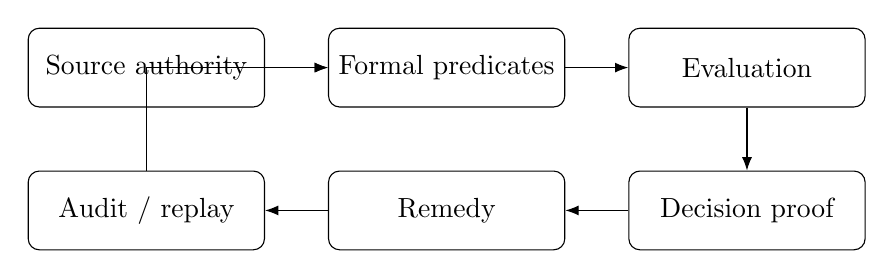
\begin{tikzpicture}[node distance=8mm, box/.style={draw,rounded corners,minimum width=30mm,minimum height=10mm,align=center}, >=Latex]
\node[box] (s) {Source authority};
\node[box,right=of s] (f) {Formal predicates};
\node[box,right=of f] (e) {Evaluation};
\node[box,below=of e] (p) {Decision proof};
\node[box,left=of p] (r) {Remedy};
\node[box,left=of r] (a) {Audit / replay};
\draw[->] (s)--(f);\draw[->] (f)--(e);\draw[->] (e)--(p);\draw[->] (p)--(r);\draw[->] (r)--(a);\draw[->] (a) |- (f);
\end{tikzpicture}
\caption{Closed-loop authority architecture.}
\end{figure}

\section{Architectural invariants}
\begin{requirement}[ACA-100-001]
A conforming implementation SHALL identify the versioned rule set used for every consequential decision.
\end{requirement}
\begin{requirement}[ACA-100-002]
A conforming implementation SHALL preserve unresolved, conflicting, expired, and revoked inputs as distinct machine-readable states.
\end{requirement}
\begin{requirement}[ACA-100-003]
A conforming implementation SHALL generate a Decision Proof Record for each completed evaluation.
\end{requirement}
\begin{requirement}[ACA-100-004]
A conforming implementation SHALL expose at least one defined remedy or review route for every non-final or adverse state.
\end{requirement}

\chapter{ACA-110 --- Core Terminology}
\begin{longtable}{>{\bfseries}p{0.25\textwidth}p{0.68\textwidth}}
Authority object & Versioned representation of the claimed source, scope, delegate, jurisdiction, effective period, and revocation status of authority.\\
Evidence object & Referenced assertion or artifact with provenance, integrity metadata, access controls, and status.\\
Predicate & Typed proposition evaluated under a declared rule version.\\
Verifiable Authority Cell & Reusable decision primitive that evaluates mandatory predicates and emits a defined decision state.\\
Decision Proof Record & Portable record sufficient to inspect and independently replay an evaluation, subject to lawful access controls.\\
Operationalized remedy & Defined, time-bounded process for notice, review, correction, propagation, verification, and closure.\\
Authority Transistor & Public metaphor for the smallest reusable authority-control element; not a claim of a novel semiconductor device.\\
\end{longtable}

\chapter{ACA-120 --- Verifiable Authority Cell}

\section{Scope}
This chapter defines the normative contract for a Verifiable Authority Cell
(VAC). A VAC is the smallest reusable ACA decision primitive that evaluates a
declared set of authority, jurisdiction, rule, evidence, procedure, time,
notice, conflict, and prohibition predicates and emits a canonical decision
state with sufficient proof and remedy metadata for independent inspection.

A conforming VAC does not determine whether an assertion is true merely because
it is well formed, signed, or hashed. It evaluates declared inputs under a
versioned profile and records the basis, limits, and consequences of that
evaluation.

\section{Conformance language}
The key words SHALL, SHALL NOT, SHOULD, SHOULD NOT, and MAY are to be
interpreted as normative requirements. A deployment claiming ACA-120
conformance SHALL identify the profile, schema version, rule version,
evaluator version, and conformance-test version used for each evaluation.

\begin{requirement}[ACA-120-001]
A conforming implementation SHALL satisfy every applicable SHALL and SHALL NOT
requirement in this chapter and SHALL produce evidence sufficient to verify that
claim.
\end{requirement}

\begin{requirement}[ACA-120-002]
A profile MAY add constraints or safe states, but it SHALL NOT weaken a baseline
safety requirement, erase provenance, reinterpret a canonical state, or permit
an action that the baseline contract requires to be held, denied, revoked, or
escalated.
\end{requirement}

\section{Authority Cell identity and boundary}
Each VAC evaluation SHALL have a unique cell identifier and evaluation
identifier. The cell identifier names the reusable decision primitive; the
evaluation identifier names one execution of that primitive.

\begin{requirement}[ACA-120-003]
The cell boundary SHALL declare its inputs, outputs, governing profile,
authoritative rule sources, required evidence classes, permitted callers,
permitted downstream actions, and remedy route.
\end{requirement}

\begin{requirement}[ACA-120-004]
Inputs not declared by the governing profile SHALL NOT silently influence the
evaluation. Any external human or automated influence SHALL be represented as a
versioned input, override, or review event.
\end{requirement}

\section{Canonical predicate model}
A baseline cell evaluates:
\[
I=\{A,J,R,E,P,T,N,C,V\}
\]
where $A$ is authority validity, $J$ jurisdiction, $R$ rule applicability, $E$
evidence sufficiency, $P$ required procedure, $T$ temporal validity, $N$ notice
and review, $C$ conflict state, and $V$ revocation or prohibition.

Each material predicate SHALL include:
\begin{enumerate}
\item a stable predicate identifier;
\item a declared type and value domain;
\item whether it is mandatory or advisory;
\item the rule or profile provision that requires it;
\item its evaluated value;
\item the evidence or authority references used;
\item the evaluator identity and evaluation time;
\item its confidence, uncertainty, or non-computability status where applicable;
\item an explanation code suitable for testing and review.
\end{enumerate}

\begin{requirement}[ACA-120-005]
Predicate values SHALL be drawn from a declared finite domain. The baseline
domain SHALL distinguish at least \state{TRUE}, \state{FALSE},
\state{UNKNOWN}, \state{CONFLICTED}, and \state{NOT-APPLICABLE}.
\end{requirement}

\begin{requirement}[ACA-120-006]
A mandatory predicate with value \state{UNKNOWN} SHALL prevent
\state{ALLOW}.
\end{requirement}

\begin{requirement}[ACA-120-007]
A mandatory predicate with value \state{CONFLICTED} SHALL produce
\state{CONFLICT} unless a profile defines a higher-priority safe state.
\end{requirement}

\begin{requirement}[ACA-120-008]
\state{NOT-APPLICABLE} SHALL be permitted only when the governing profile
contains an explicit applicability rule that can be independently evaluated.
It SHALL NOT be used as a substitute for missing evidence or unresolved scope.
\end{requirement}

\begin{requirement}[ACA-120-009]
Profiles SHALL identify which predicates are objective, evidentiary,
discretionary, or non-computable. Human judgment SHALL NOT be concealed as
deterministic computation.
\end{requirement}

\section{Authority and jurisdiction binding}
The authority object and jurisdiction predicate establish who may decide what,
for whom, where, during what period, and subject to which delegation,
prohibition, and review structure.

\begin{requirement}[ACA-120-010]
An authority reference SHALL identify the claimed source, issuer, delegate,
scope, affected subject or resource class, jurisdiction, effective period,
version, and revocation status.
\end{requirement}

\begin{requirement}[ACA-120-011]
A delegation SHALL NOT convey broader scope, longer duration, greater remedy
immunity, or higher precedence than the delegating authority possesses.
\end{requirement}

\begin{requirement}[ACA-120-012]
The subject, resource, transaction, or decision target evaluated by the cell
SHALL be explicitly bound to the authority and jurisdiction inputs. Name,
identifier, role, or record similarity alone SHALL NOT establish that binding.
\end{requirement}

\begin{requirement}[ACA-120-013]
Where authority or jurisdiction depends on a disputed fact, the dependency
SHALL be represented as a material predicate and SHALL NOT be assumed by the
evaluator.
\end{requirement}

\section{Rule and profile binding}
A VAC evaluates a declared rule set rather than an unversioned narrative.

\begin{requirement}[ACA-120-014]
Every evaluation SHALL bind to an immutable rule version and profile version.
A later rule change SHALL NOT retroactively alter the recorded result of an
earlier evaluation; it SHALL create a new evaluation or review event.
\end{requirement}

\begin{requirement}[ACA-120-015]
The profile SHALL declare predicate dependencies, mandatory predicates,
precedence rules, state-resolution rules, permitted overrides, and remedy
obligations in a form suitable for conformance testing.
\end{requirement}

\begin{requirement}[ACA-120-016]
Free-form prose MAY accompany a rule or predicate, but prose alone SHALL NOT be
treated as executable semantics when a conformance claim depends on that
semantics.
\end{requirement}

\section{Evidence sufficiency and provenance}
Evidence sufficiency is profile-relative and SHALL remain distinct from evidence
integrity and factual truth.

\begin{requirement}[ACA-120-017]
Each material evidence reference SHALL identify provenance, acquisition time,
source identity or source class, integrity metadata, access restrictions,
status, and the assertion it is offered to support or contradict.
\end{requirement}

\begin{requirement}[ACA-120-018]
A hash, signature, timestamp, or chain-of-custody record MAY support integrity
or attribution, but SHALL NOT by itself be treated as proof that the underlying
assertion is true, complete, lawful, or applicable.
\end{requirement}

\begin{requirement}[ACA-120-019]
The evaluator SHALL record material evidence that supports, contradicts, limits,
or remains unavailable for a predicate. Selective omission of known material
contradictory evidence is non-conforming.
\end{requirement}

\begin{requirement}[ACA-120-020]
Where lawful access restrictions prevent disclosure, the Decision Proof Record
SHALL preserve the existence, class, custodian, access rule, and effect of the
restricted evidence without exposing protected content.
\end{requirement}

\section{Procedure, notice, and review}
Procedure and notice are independently testable authorization conditions, not
post-decision annotations.

\begin{requirement}[ACA-120-021]
A required procedural step SHALL identify its responsible actor, triggering
condition, permitted sequence, completion evidence, deadline, and consequence
of non-completion.
\end{requirement}

\begin{requirement}[ACA-120-022]
Where notice or review is required before authorization or execution, absent,
untimely, defective, or unverified notice SHALL prevent \state{ALLOW} unless a
published profile defines a lawful emergency path and its additional safeguards.
\end{requirement}

\begin{requirement}[ACA-120-023]
An emergency path SHALL be explicit, time-bounded, independently reviewable, and
incapable of silently becoming the ordinary path.
\end{requirement}

\section{Temporal validity}
Time SHALL be evaluated as part of authority, rule, evidence, procedure, and
remedy validity.

\begin{requirement}[ACA-120-024]
The evaluator SHALL record the evaluation time, applicable effective intervals,
expiration conditions, and the clock or trusted time source used where time is
material.
\end{requirement}

\begin{requirement}[ACA-120-025]
Expired authority, expired evidence where freshness is mandatory, or an expired
procedural window SHALL prevent \state{ALLOW} unless the governing profile
contains an explicit and testable exception.
\end{requirement}

\section{Conflict, prohibition, and revocation precedence}
For profiles that permit Boolean authorization, the baseline allow expression
is:
\[
\state{ALLOW}=A\land J\land R\land E\land P\land T\land N\land \neg C\land \neg V.
\]
This expression is a minimum authorization condition, not a complete execution
instruction.

\begin{requirement}[ACA-120-026]
A valid revocation or prohibition SHALL take precedence over ordinary
authorization.
\end{requirement}

\begin{requirement}[ACA-120-027]
A conflict SHALL identify the conflicting assertions, authorities, rules, or
evidence objects and the precedence rule, review route, or missing fact required
to resolve it.
\end{requirement}

\begin{requirement}[ACA-120-028]
An implementation SHALL NOT resolve a conflict by discarding the lower-ranked
or inconvenient input from the proof record.
\end{requirement}

\section{Decision states and resolution}
A VAC SHALL emit one canonical state defined by ACA-130:
\[
S\in\{\state{ALLOW},\state{DENY},\state{HOLD},\state{CONFLICT},
\state{REVOKED},\state{ESCALATE}\}.
\]

\begin{requirement}[ACA-120-029]
\state{ALLOW} SHALL require every mandatory positive authorization predicate to
be satisfied and every mandatory conflict, revocation, or prohibition predicate
to be cleared.
\end{requirement}

\begin{requirement}[ACA-120-030]
\state{DENY} SHALL identify at least one evaluated rule condition that affirmatively
requires denial. Missing information alone SHALL ordinarily produce
\state{HOLD} or \state{ESCALATE}, not \state{DENY}.
\end{requirement}

\begin{requirement}[ACA-120-031]
\state{HOLD} SHALL identify the unresolved predicate, required evidence or
procedure, responsible route, and applicable deadline.
\end{requirement}

\begin{requirement}[ACA-120-032]
\state{ESCALATE} SHALL identify why the cell cannot safely or lawfully resolve
the evaluation and the qualified human or higher-order authority authorized to
review it.
\end{requirement}

\begin{requirement}[ACA-120-033]
Every emitted state SHALL include a stable reason code and a human-readable
explanation that is consistent with the recorded predicates and precedence
rules.
\end{requirement}

\section{Authorization and execution separation}
An authorization decision and the execution of an action are distinct events.

\begin{requirement}[ACA-120-034]
A VAC SHALL NOT represent an authorized decision as executed unless a separate
execution record identifies the action, executor, time, target, authorization
reference, result, and integrity mechanism.
\end{requirement}

\begin{requirement}[ACA-120-035]
Before execution, the executing component SHALL verify that the authorization
remains current, unrevoked, applicable to the target, and within any declared
execution window.
\end{requirement}

\begin{requirement}[ACA-120-036]
A failed, partial, delayed, duplicated, or reversed execution SHALL be recorded
without rewriting the original authorization decision.
\end{requirement}

\section{Decision Proof Record}
Every evaluation SHALL emit or reference a Decision Proof Record conforming to
ACA-140.

\begin{requirement}[ACA-120-037]
The proof record SHALL contain the cell and evaluation identifiers, profile and
rule versions, evaluator identity, material inputs, predicate results, emitted
state, reason code, conflicts and unknowns, authority and evidence references,
remedy route, and integrity metadata.
\end{requirement}

\begin{requirement}[ACA-120-038]
The proof record SHALL preserve sufficient normalized input and configuration
metadata to permit deterministic replay when the evaluator has lawful access to
the same versions and evidence objects.
\end{requirement}

\begin{requirement}[ACA-120-039]
The record SHALL distinguish an integrity proof, an attribution proof, an
authority evaluation, and a factual truth claim. None SHALL be silently
substituted for another.
\end{requirement}

\section{Replay and determinism}

\begin{requirement}[ACA-120-040]
A conforming implementation SHALL declare its canonicalization rules for object
ordering, numeric representation, text normalization, time representation,
identifier comparison, omitted values, and cryptographic digest construction.
\end{requirement}

\begin{requirement}[ACA-120-041]
Given the same normalized inputs, rule version, profile version, evaluator
version, and permitted deterministic dependencies, replay SHALL produce the
same predicate values, state, and reason code.
\end{requirement}

\begin{requirement}[ACA-120-042]
Non-deterministic services, probabilistic models, or mutable external data MAY
inform a predicate only when their identity, version, input, output, uncertainty,
and review rule are recorded. Their output SHALL NOT be mislabeled as
deterministic replay evidence.
\end{requirement}

\section{Remedy attachment}
A terminal or adverse state does not complete the ACA lifecycle unless the
applicable remedy is defined.

\begin{requirement}[ACA-120-043]
Every \state{DENY}, \state{HOLD}, \state{CONFLICT}, \state{REVOKED}, or
\state{ESCALATE} state SHALL identify an available remedy or shall explicitly
record that no remedy is provided, by what authority, and subject to what review.
\end{requirement}

\begin{requirement}[ACA-120-044]
A remedy reference SHALL identify the responsible authority, permitted filer or
initiator, required inputs, deadline, review sequence, correction mechanism,
propagation obligations, verification condition, and closure rule.
\end{requirement}

\begin{requirement}[ACA-120-045]
A later correction SHALL preserve the original evaluation and create a linked
correction, propagation, and verification history conforming to ACA-150.
\end{requirement}

\section{Security and abuse resistance}

\begin{requirement}[ACA-120-046]
Implementations SHALL enforce least privilege for evaluation, review, override,
execution, evidence access, and remedy closure. Possession of write access to
one function SHALL NOT imply authority to perform the others.
\end{requirement}

\begin{requirement}[ACA-120-047]
Overrides SHALL identify the authorized actor, legal or policy basis, scope,
reason, time, affected predicates, resulting state, expiration, and required
independent review. Undocumented override behavior is non-conforming.
\end{requirement}

\begin{requirement}[ACA-120-048]
The implementation SHALL detect or prevent replay substitution, stale authority,
identifier collision, unauthorized profile changes, evidence-reference
replacement, and suppression of material conflicts to the extent required by
the deployment threat model.
\end{requirement}

\begin{requirement}[ACA-120-049]
Sensitive evidence and personal data SHALL be minimized and access-controlled,
but minimization SHALL NOT erase the proof that a material input existed or
alter its recorded effect on the decision.
\end{requirement}

\section{Conformance evidence and traceability}

\begin{requirement}[ACA-120-050]
Each normative requirement claimed by an implementation SHALL map to at least
one specification reference, implementation control, positive test, negative or
adversarial test where applicable, and retained test result.
\end{requirement}

\begin{requirement}[ACA-120-051]
A schema-valid object SHALL NOT be labeled substantively conforming unless its
cross-object bindings, predicate semantics, state resolution, proof record,
replay behavior, and remedy obligations also pass the applicable conformance
suite.
\end{requirement}

\begin{requirement}[ACA-120-052]
A conformance report SHALL identify every requirement tested, passed, failed,
not applicable, or not tested. Partial conformance SHALL be labeled as partial
and SHALL NOT be presented as full ACA-120 conformance.
\end{requirement}

\section{Versioning and extension rules}

\begin{requirement}[ACA-120-053]
Every extension predicate, state restriction, evidence class, or precedence rule
SHALL use a collision-resistant identifier and SHALL declare its relationship to
the baseline contract.
\end{requirement}

\begin{requirement}[ACA-120-054]
A breaking semantic change SHALL require a new contract or profile version and
SHALL NOT be introduced solely by changing prose, examples, evaluator code, or
an external service.
\end{requirement}

\begin{requirement}[ACA-120-055]
Deprecated fields or rules SHALL remain interpretable for the declared retention
period, and migrations SHALL preserve the original version, meaning, proof
record, and remedy history.
\end{requirement}

\section{Minimum acceptance criteria}
An ACA-120 candidate is eligible for approval only when:
\begin{enumerate}
\item the normative text is versioned and reviewable;
\item the Authority Cell schema expresses the required structural contract;
\item positive, negative, conflict, revocation, expiration, unknown, override,
and replay examples exist;
\item a requirement-to-schema-to-test traceability matrix exists;
\item the conformance suite verifies state resolution and fail-safe behavior;
\item authorization and execution are represented separately;
\item proof-record and remedy obligations are tested; and
\item all known deviations are documented as explicit, time-bounded exceptions.
\end{enumerate}

This chapter defines the normative Authority Cell contract. ACA-130 defines the
state-machine transitions, ACA-140 defines the portable Decision Proof Record,
and ACA-150 defines the remedy lifecycle that follows an unresolved, adverse,
revoked, or corrected decision.
\chapter{ACA-130 --- Decision State Machine}
\section{Canonical states}
\[
S\in\{\state{ALLOW},\state{DENY},\state{HOLD},\state{CONFLICT},\state{REVOKED},\state{ESCALATE}\}.
\]

\begin{figure}[ht]
\centering
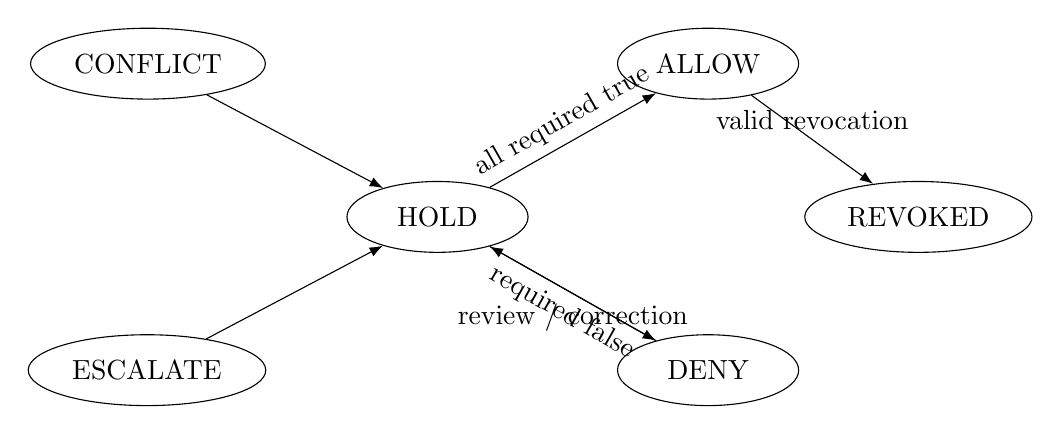
\begin{tikzpicture}[node distance=13mm and 18mm, st/.style={draw,ellipse,minimum width=23mm,minimum height=9mm}, >=Latex]
\node[st] (hold) {HOLD};
\node[st,above right=of hold] (allow) {ALLOW};
\node[st,below right=of hold] (deny) {DENY};
\node[st,above left=of hold] (conf) {CONFLICT};
\node[st,below left=of hold] (esc) {ESCALATE};
\node[st,right=35mm of hold] (rev) {REVOKED};
\draw[->] (hold)--node[above,sloped]{all required true}(allow);
\draw[->] (hold)--node[below,sloped]{required false}(deny);
\draw[->] (conf)--(hold);
\draw[->] (esc)--(hold);
\draw[->] (allow)--node[above]{valid revocation}(rev);
\draw[->] (deny)--node[below]{review / correction}(hold);
\end{tikzpicture}
\caption{Baseline state transitions. Profiles may restrict transitions but may not erase provenance.}
\end{figure}

\begin{requirement}[ACA-130-001]
Every transition SHALL record its triggering event, actor or service identity, timestamp, prior state, resulting state, and rule version.
\end{requirement}

\chapter{ACA-140 --- Decision Proof Record}
\section{Minimum record}
A Decision Proof Record SHALL contain:
\begin{enumerate}
\item a unique record identifier;
\item the decision profile and rule version;
\item evaluation time and implementation identity;
\item each material predicate, value, source, and evidence reference;
\item the final state and transition reason;
\item identified conflicts, unknowns, expirations, and revocations;
\item the available remedy route and applicable deadline;
\item an integrity mechanism suitable to the deployment context.
\end{enumerate}

\begin{requirement}[ACA-140-001]
The record SHALL support deterministic replay when the evaluator has lawful access to the same rule versions and evidence objects.
\end{requirement}
\begin{requirement}[ACA-140-002]
The record SHALL distinguish integrity proof from truth proof. A cryptographic hash proves that content has not changed; it does not prove that the original assertion was true.
\end{requirement}

\chapter{ACA-150 --- Operationalized Remedy Protocol}
\section{Lifecycle}
The baseline remedy lifecycle is:
\[
\text{Detect}\rightarrow\text{Notify}\rightarrow\text{Preserve}\rightarrow
\text{Review}\rightarrow\text{Correct}\rightarrow\text{Propagate}\rightarrow
\text{Verify}\rightarrow\text{Close}.
\]

\begin{requirement}[ACA-150-001]
A remedy SHALL NOT be marked complete merely because a review occurred.
\end{requirement}
\begin{requirement}[ACA-150-002]
Closure SHALL require evidence that the corrective action was executed and, where applicable, propagated to dependent records and downstream decisions.
\end{requirement}
\begin{requirement}[ACA-150-003]
The protocol SHALL retain the original state, correction history, responsible authority, elapsed time, and verification result.
\end{requirement}

\section{Core measures}
Deployments SHOULD report: decision reproducibility rate, unresolved-input rate, contradiction-detection rate, median correction time, remedy completion rate, downstream propagation completeness, and independent replay success.

\chapter{ACA-160 --- Predicate Failure Taxonomy}

\section{Purpose}
This chapter defines a diagnostic taxonomy for failures of the nine canonical predicates evaluated by the Verifiable Authority Cell (VAC) in ACA-120. It does not replace the predicate model. It classifies how a predicate can become unreliable, misleading, unavailable, improperly satisfied, or unsafe to use.

The taxonomy is intended for conformance testing, adversarial testing, incident analysis, corrective action, and remedy design. It classifies observable system conditions rather than presumed motives or moral character.

\begin{requirement}[ACA-160-001]
A claimed predicate failure SHALL identify the affected predicate, failure mode, observable indicators, supporting evidence, decision effect, propagation scope, and available containment or remedy.
\end{requirement}

\begin{requirement}[ACA-160-002]
A failure classification SHALL NOT by itself establish unlawful conduct, malicious intent, factual falsity, or legal invalidity. Those conclusions require independent evidence and the applicable governing standard.
\end{requirement}

\section{Taxonomy structure}
Each failure entry uses the following fields:
\begin{enumerate}
\item \textbf{Code}: stable identifier;
\item \textbf{Predicate}: one of $A,J,R,E,P,T,N,C,V$;
\item \textbf{Failure mode}: the structural defect;
\item \textbf{Trigger or cause}: how the defect may arise;
\item \textbf{Observable indicators}: evidence suitable for testing;
\item \textbf{Decision effect}: expected effect on the VAC state;
\item \textbf{Propagation risk}: how later cells or records may inherit the defect;
\item \textbf{Containment}: immediate action to prevent additional reliance;
\item \textbf{Remedy}: correction, review, restoration, or closure path.
\end{enumerate}

\section{Cross-cutting failure classes}
\begin{longtable}{p{0.18\textwidth}p{0.30\textwidth}p{0.42\textwidth}}
\toprule
\textbf{Class} & \textbf{Definition} & \textbf{Baseline response}\\
\midrule
\endfirsthead
\toprule
\textbf{Class} & \textbf{Definition} & \textbf{Baseline response}\\
\midrule
\endhead
Missing & A mandatory predicate was not evaluated or its required object is absent. & Prevent \state{ALLOW}; ordinarily emit \state{HOLD} or \state{ESCALATE}.\\
Unsupported & A value is asserted without the evidence or rule reference required by the profile. & Mark \state{UNKNOWN}; request the missing support.\\
Misbound & Valid information is attached to the wrong subject, action, jurisdiction, rule, time, or authority object. & Quarantine the affected evaluation and test all downstream bindings.\\
Stale & The value was once usable but its effective interval, evidence freshness, delegation, or review period has expired. & Re-evaluate from current sources; prevent execution.\\
Conflicted & Material sources support incompatible values and no valid precedence rule resolves them. & Emit \state{CONFLICT}; preserve all competing inputs.\\
Substituted & One proof type is silently used as another, such as integrity being treated as truth or status as authorization. & Reject the substitution and evaluate the actual required predicate.\\
Suppressed & Known material contrary, limiting, or revoking information is omitted from evaluation or proof. & Suspend reliance; restore the omitted input and replay.\\
Overridden & A value or state is changed outside the declared override authority, scope, or review process. & Treat as non-conforming; revoke or hold the resulting action pending review.\\
Ambiguous & The predicate, value domain, rule, target, or reason code permits materially different interpretations. & Escalate for clarification; version the corrected definition.\\
Non-replayable & The result cannot be reproduced from retained inputs, versions, and declared dependencies. & Mark conformance unproven and preserve the original record for investigation.\\
\bottomrule
\end{longtable}

\section{Authority validity failures ($A$)}
\begin{description}[style=nextline]
\item[A-USURPATION --- Unestablished authority exercised]
An actor or component exercises power without a demonstrated source and chain. Indicators include absent source authority, missing delegation, or action beyond declared scope. Baseline effect: \state{DENY}, \state{HOLD}, or \state{ESCALATE}; never \state{ALLOW}.

\item[A-LAUNDERING --- Unsupported assertion converted into apparent authority]
A private, informal, automated, or unverified assertion is incorporated into an official record and later relied upon as if its authority were independently established. Containment requires marking the derived records, stopping further reliance, and tracing every dependent evaluation.

\item[A-SCOPE-DRIFT --- Authority exceeds delegated scope]
The actor, subject, action, duration, remedy, or territory exceeds the source authority.

\item[A-STATUS-SUBSTITUTION --- Role or title treated as action-specific authorization]
A person's office, credential, employment, or institutional status is treated as sufficient without evaluating the predicates for the particular action.

\item[A-BROKEN-CHAIN --- Delegation path is incomplete]
One or more links between source authority and the acting component are absent, expired, inconsistent, or unverifiable.
\end{description}

\section{Jurisdiction failures ($J$)}
\begin{description}[style=nextline]
\item[J-NEXUS-FAILURE --- Required connection not established]
The record does not establish the required relationship between the decision and the forum, subject, resource, transaction, or matter.

\item[J-TARGET-MISBINDING --- Jurisdiction attached to the wrong target]
Identifiers, names, records, or roles are confused, merged, or assumed equivalent.

\item[J-BOUNDARY-EXPANSION --- Jurisdiction silently broadened]
A narrow or emergency basis is used to support ordinary, continuing, or broader power without a fresh evaluation.

\item[J-COMPETING-FORUM-SUPPRESSION --- Material competing jurisdiction omitted]
A potentially controlling or conflicting forum, rule, or authority is not represented in the conflict analysis.
\end{description}

\section{Rule applicability failures ($R$)}
\begin{description}[style=nextline]
\item[R-WRONG-RULE --- Non-governing rule selected]
A rule is authentic but does not govern the subject, event, actor, or requested remedy.

\item[R-VERSION-DRIFT --- Unversioned or incorrect rule version used]
The evaluator cannot identify the exact rule text and effective version used.

\item[R-EXCEPTION-SUPPRESSION --- Applicable exception omitted]
A limiting clause, exception, defense, exemption, or precedence rule is excluded from executable semantics.

\item[R-NARRATIVE-SUBSTITUTION --- Prose conclusion replaces executable rule]
A summary, label, allegation, or prior outcome is treated as the rule itself.
\end{description}

\section{Evidence sufficiency failures ($E$)}
\begin{description}[style=nextline]
\item[E-ASSERTION-AS-EVIDENCE --- Repetition treated as corroboration]
An assertion gains apparent weight through copying, citation, database entry, or institutional repetition without an independent evidentiary basis.

\item[E-INTEGRITY-AS-TRUTH --- Authenticity substituted for factual truth]
A signature, hash, timestamp, or chain of custody proves integrity or attribution but is treated as proving the underlying assertion.

\item[E-SELECTIVE-RECORD --- Material contrary evidence suppressed]
Known supporting, limiting, contradictory, unavailable, or exculpatory evidence is omitted from evaluation.

\item[E-PROVENANCE-BREAK --- Source or acquisition history cannot be verified]
The evidence object cannot be reliably connected to its origin, custodian, collection method, or asserted fact.

\item[E-THRESHOLD-DRIFT --- Sufficiency threshold changes without versioning]
The quantity or quality of evidence required for approval is changed implicitly, inconsistently, or after the fact.
\end{description}

\section{Procedure completeness failures ($P$)}
\begin{description}[style=nextline]
\item[P-SKIPPED-INTERLOCK --- Required step bypassed]
A mandatory review, verification, hearing, approval, consultation, or safeguard is omitted.

\item[P-SEQUENCE-INVERSION --- Outcome precedes prerequisite]
Execution, restriction, publication, or enforcement occurs before the procedure that authorizes it.

\item[P-RUBBER-STAMP --- Review exists in form but not function]
The designated reviewer lacks time, information, independence, competence, or real authority to reject or correct the proposed action.

\item[P-EMERGENCY-NORMALIZATION --- Exceptional path becomes ordinary]
An emergency procedure persists, expands, or repeats without renewed predicates and safeguards.
\end{description}

\section{Temporal validity failures ($T$)}
\begin{description}[style=nextline]
\item[T-STALE-AUTHORITY --- Expired authority relied upon]
A delegation, appointment, order, credential, or permission is used outside its effective interval.

\item[T-RETROACTIVE-BINDING --- Later state rewrites earlier authority]
A later rule, finding, record, or authorization is treated as if it existed when the original action occurred.

\item[T-DELAYED-REMEDY --- Review becomes functionally unavailable]
Delay prevents meaningful correction, restoration, preservation, or challenge.

\item[T-CLOCK-AMBIGUITY --- Material time cannot be established]
The evaluation lacks a trusted time source, synchronized sequence, or applicable interval.
\end{description}

\section{Notice and review failures ($N$)}
\begin{description}[style=nextline]
\item[N-NOTICE-FAILURE --- Required notice absent or defective]
Notice is missing, late, sent to the wrong recipient, inaccessible, incomplete, or does not identify the proposed action and response path.

\item[N-ILLUSORY-REVIEW --- Review exists nominally but cannot provide correction]
The reviewer lacks jurisdiction, independence, evidence access, remedial power, or sufficient time.

\item[N-BURDEN-INVERSION --- Affected party must disprove unestablished authority]
The system acts first and shifts the burden to the affected party to establish that prerequisites were never satisfied.

\item[N-REASON-SUPPRESSION --- Decision basis is not disclosed enough to challenge]
The proof record lacks the rule, predicates, evidence classes, reason code, or review instructions necessary for meaningful contest.
\end{description}

\section{Conflict failures ($C$)}
\begin{description}[style=nextline]
\item[C-HIDDEN-CONFLICT --- Material conflict not represented]
The evaluator suppresses or fails to detect an incompatible source, interest, rule, identity, or prior decision.

\item[C-SELF-REVIEW --- Conflicted actor controls resolution]
The same actor creates, evaluates, executes, and closes review of the disputed action without an independent control required by the profile.

\item[C-FALSE-PRECEDENCE --- Priority asserted without governing basis]
One source or assertion is treated as controlling without an applicable and versioned precedence rule.

\item[C-CONFLICT-COLLAPSE --- Conflict silently converted to approval]
The system discards uncertainty or contradiction rather than emitting \state{CONFLICT} or \state{ESCALATE}.
\end{description}

\section{Revocation and prohibition failures ($V$)}
\begin{description}[style=nextline]
\item[V-REVOCATION-SUPPRESSION --- Current revocation ignored]
A valid revocation exists but is absent, hidden, delayed, or treated as advisory.

\item[V-STALE-PROHIBITION --- Expired restriction treated as current]
A prior prohibition continues to block action after its valid period or scope.

\item[V-OVERRIDDEN-BAR --- Prohibition bypassed without valid override]
The override actor, scope, basis, duration, or independent review is missing.

\item[V-PROPAGATION-FAILURE --- Revocation does not reach dependent systems]
Downstream cells, records, permissions, or executions continue relying on the revoked object.
\end{description}

\section{Propagation taxonomy}
A local predicate failure becomes systemic when dependent decisions inherit it without re-evaluation.

\begin{description}[style=nextline]
\item[PR-COPY] A defective assertion is copied into additional records.
\item[PR-CITATION] Later decisions cite the defective record as independent support.
\item[PR-AUTOMATION] Software repeatedly applies the defective value at scale.
\item[PR-CREDENTIAL] The defective outcome creates a role, permission, restriction, or status used as a new input.
\item[PR-PRECEDENT] A prior defective outcome is treated as a controlling template.
\item[PR-REMEDY-BLOCK] The propagated state obstructs the route needed to correct its own source.
\end{description}

\begin{requirement}[ACA-160-003]
When a material predicate failure is confirmed, the responsible system SHALL identify all reasonably discoverable dependent cells, proof records, executions, credentials, restrictions, and remedies that relied on the failed value.
\end{requirement}

\section{Containment and recovery}
\begin{enumerate}
\item mark the affected predicate and evaluation as disputed, invalid, stale, or under review;
\item prevent new \state{ALLOW} decisions that depend on the failed value;
\item preserve the original proof and execution history;
\item identify the smallest compromised unit and all downstream dependencies;
\item obtain or re-evaluate the missing source, evidence, rule, procedure, time, notice, conflict, or revocation input;
\item replay affected cells under corrected and versioned inputs;
\item reverse, amend, compensate, notify, or otherwise remedy affected outputs under ACA-150;
\item verify propagation and closure independently.
\end{enumerate}

\begin{requirement}[ACA-160-004]
Correction SHALL create a linked, append-only history. It SHALL NOT erase the original predicate value, decision, execution, or impact.
\end{requirement}

\begin{requirement}[ACA-160-005]
A failure SHALL remain open until the source defect, dependent evaluations, executed consequences, affected parties, and required remedies have each been resolved or explicitly recorded as unresolved by an identified authority.
\end{requirement}

\section{Initial conformance tests}
A conforming test suite SHOULD include at least:
\begin{enumerate}
\item one positive baseline for every predicate;
\item one missing, unsupported, misbound, stale, conflicted, substituted, suppressed, and overridden case;
\item one case in which an unsupported assertion is copied into a later record;
\item one case in which status is incorrectly substituted for authorization;
\item one case in which a revocation fails to propagate;
\item one case in which an emergency path attempts to become permanent;
\item one remedy replay showing correction without deletion of history.
\end{enumerate}

\section{Design rule}
\begin{requirement}[ACA-160-006]
A system SHALL NOT treat repetition, institutional possession, procedural completion, technical integrity, actor status, or prior execution as independent proof that the predicates required for present authorization are satisfied.
\end{requirement}

\chapter{Implementation Roadmap}
\section{First bounded profile}
The first reference implementation should address a narrow decision with published rules, objective evidence, limited discretion, and a clear correction path. A filing-completeness or deadline-validity profile is preferable to a high-discretion adjudication.

\section{Acceptance tests}
The first implementation is not accepted until:
\begin{enumerate}
\item repeated evaluation of identical inputs produces identical records;
\item two independent implementations produce equivalent states and reasons;
\item missing evidence cannot produce \state{ALLOW};
\item conflicting evidence is visibly preserved;
\item revocation propagates to dependent decisions;
\item every adverse or incomplete result identifies a testable remedy route.
\end{enumerate}

\section{Strategic outputs}
The program should publish, in order: architecture, terminology, cell specification, state machine, proof schema, remedy protocol, test fixtures, reference implementation, independent evaluation, and conformance profile.

\appendix
\chapter{Minimal Decision Proof Record}
\begin{verbatim}
{
  "record_id": "DPR-example-0001",
  "state": "HOLD",
  "predicates": [
    {"id":"authority.valid","value":"TRUE"},
    {"id":"evidence.complete","value":"UNKNOWN"}
  ],
  "remedy": {"status":"AVAILABLE","route":"supply-missing-evidence"}
}
\end{verbatim}
\end{document}
